% Copyright (c) 2021-2023 Eclipse Arrowhead Project
%
% This program and the accompanying materials are made available under the
% terms of the Eclipse Public License 2.0 which is available at
% http://www.eclipse.org/legal/epl-2.0.
%
% SPDX-License-Identifier: EPL-2.0

With the major themes of the \GlossaryHyperRef{framework-arrowhead}{Arrowhead framework} now established, we are ready to define its primary concepts more rigorously.
To begin with, we summarize the concepts in Table \ref{tab:concepts:summary}, which presents the categories they fall into, the sections they appear in, their names, as well as summaries of their definitions.
You may choose to read the table from beginning to end, use it as a means of deciding what concepts to read more about, or simply skip it if you feel the repetition is unnecessary.

\begin{table}[ht!]
\noindent\begin{tabularx}{\textwidth}{@{} p{0.2cm} p{0.7cm} p{4.3cm} X @{}}

\multicolumn{3}{@{} p{5.2cm} @{}}{\textbf{Fundamental Concepts}}               & \textit{The foundation upon which all other primary concepts are defined.} \\ [2mm]
& \ref{sec:concepts:stakeholder} & \textbf{\nameref{sec:concepts:stakeholder}} & A person or \GlossaryHyperRef{organization}{organization} concerned with an \GlossaryHyperRef{entity}{entity} or undertaking. \\
& \ref{sec:concepts:entity}      & \textbf{\nameref{sec:concepts:entity}}      & An \GlossaryHyperRef{artifact}{artifact} that can be distinguished from all other artifacts. \\
&&&\\
\multicolumn{3}{@{} p{5.2cm} @{}}{\textbf{Systemic Concepts}}                  & \textit{The primary building blocks of Arrowhead.} \\ [2mm]
& \ref{sec:concepts:device}      & \textbf{\nameref{sec:concepts:device}}      & A physical \GlossaryHyperRef{entity}{entity} with the \GlossaryHyperRef{capability}{capability} of hosting \GlossaryHyperRef{system}{systems}. \\
& \ref{sec:concepts:system}      & \textbf{\nameref{sec:concepts:system}}      & A \GlossaryHyperRef{instance-software}{software instance} able to exercise the \GlossaryHyperRef{capability}{capabilities} of its hosting \GlossaryHyperRef{device}{device}. \\
& \ref{sec:concepts:service}     & \textbf{\nameref{sec:concepts:service}}     & A set of \GlossaryHyperRef{operation}{operations} \GlossaryHyperRef{provider-service}{provided} by a \GlossaryHyperRef{system}{system} for other systems to \GlossaryHyperRef{consumer-service}{consume}. \\
& \ref{sec:concepts:operation}   & \textbf{\nameref{sec:concepts:operation}}   & A \GlossaryHyperRef{component-software}{component} of a \GlossaryHyperRef{service}{service} that handles \GlossaryHyperRef{message}{messages}. \\
&&&\\
\multicolumn{3}{@{} p{5.2cm} @{}}{\textbf{Compositional Concepts}}             & \textit{Significant compositions of systemic concepts.} \\ [2mm]
& \ref{sec:concepts:sos}         & \textbf{\nameref{sec:concepts:sos}}         & A set of \GlossaryHyperRef{system}{systems} that collaborate by \GlossaryHyperRef{consumer-service}{consuming} each others' \GlossaryHyperRef{service}{services}. \\
& \ref{sec:concepts:cloud}       & \textbf{\nameref{sec:concepts:cloud}}       & A \GlossaryHyperRef{system-of-systems}{system-of-systems} with a \GlossaryHyperRef{boundary}{boundary} and its own \GlossaryHyperRef{resource}{resources}. \\
& \ref{sec:concepts:soc}         & \textbf{\nameref{sec:concepts:soc}}         & A set of \GlossaryHyperRef{cloud}{clouds} that collaborate by \GlossaryHyperRef{consumer-service}{consuming} each others' \GlossaryHyperRef{service}{services}. \\
&&&\\
\multicolumn{3}{@{} p{5.2cm} @{}}{\textbf{Communicational Concepts}}           & \textit{Building blocks for communication between systemic concepts.} \\ [2mm]
& \ref{sec:concepts:network}     & \textbf{\nameref{sec:concepts:network}}     & A set of \GlossaryHyperRef{device}{devices} with \GlossaryHyperRef{interface-network}{network interfaces} that are able to \GlossaryHyperRef{communication}{communicate}. \\
& \ref{sec:concepts:interface}   & \textbf{\nameref{sec:concepts:interface}}   & A \GlossaryHyperRef{boundary}{boundary} that can be crossed by the \GlossaryHyperRef{message}{messages} of certain \GlossaryHyperRef{protocol}{protocols}. \\
& \ref{sec:concepts:protocol}    & \textbf{\nameref{sec:concepts:protocol}}    & A \GlossaryHyperRef{description}{description} of what \GlossaryHyperRef{message}{messages} can be sent between certain \GlossaryHyperRef{interface}{interfaces}. \\
& \ref{sec:concepts:message}     & \textbf{\nameref{sec:concepts:message}}     & A description of how to invoke a certain \GlossaryHyperRef{service}{service} \GlossaryHyperRef{operation}{operation}. \\
& \ref{sec:concepts:policy}      & \textbf{\nameref{sec:concepts:policy}}      & A set of \GlossaryHyperRef{constraint}{constraints} that must be satisfied for a \GlossaryHyperRef{message}{message} to be \GlossaryHyperRef{message-permitted}{permitted}. \\
& \ref{sec:concepts:profile}     & \textbf{\nameref{sec:concepts:profile}}     & A set of \GlossaryHyperRef{constraint}{constraints} added to a \GlossaryHyperRef{protocol}{protocol}. \\
&&&\\
\multicolumn{3}{@{} p{5.2cm} @{}}{\textbf{Interpretational Concepts}}          & \textit{Constructs relevant to the formulation and interpretation of messages.} \\ [2mm]
& \ref{sec:concepts:encoding}    & \textbf{\nameref{sec:concepts:encoding}}    & A \GlossaryHyperRef{type-data}{data type} used to \GlossaryHyperRef{encode}{encode} and \GlossaryHyperRef{decode}{decode} \GlossaryHyperRef{data}{data}. \\
& \ref{sec:concepts:semantics}   & \textbf{\nameref{sec:concepts:semantics}}   & A \GlossaryHyperRef{model}{model} used to derive meaning from \GlossaryHyperRef{data}{data}. \\

\end{tabularx}
\caption{A summary of the primary concepts outlined in this section.}
\label{tab:concepts:summary}
\end{table}

We now proceed to present the primary concepts in the same order they appear in Table \ref{tab:concepts:summary}.

\newpage

\subsection{Stakeholder}
\label{sec:concepts:stakeholder}

A \GlossaryHyperRef{stakeholder}{stakeholder} is a person or \GlossaryHyperRef{organization}{organization} with \GlossaryHyperRef{stake}{stake} in an \GlossaryHyperRef{entity}{entity} or undertaking with relevance to the \GlossaryHyperRef{framework-arrowhead}{Arrowhead framework}, where \textit{stake} is any form of engagement or commitment.
Stake may be concretely expressed by a stakeholder being associated with one or more \GlossaryHyperRef{role-stakeholder}{\textit{roles}}, as illustrated in Figure \ref{fig:stakeholder}.

\begin{figure}[ht!]
  \centering
  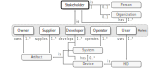
\includegraphics[scale=0.9]{figures/stakeholder}
  \caption{
    The stakeholder as either a person or organization, where each such stakeholder takes on one ore more distinct roles.
    The depicted roles are only possible examples.
    \GlossaryHyperRef{hid}{HID} is an abbreviation for \GlossaryHyperRef{device-human-interface}{Human Interface Device}.
  }
  \label{fig:stakeholder}
\end{figure}

The roles of a given stakeholder dictates what \GlossaryHyperRef{entity}{entities} that person or organization will interact with, as well as the nature of those interactions.
In Figure \ref{fig:stakeholder}, (1) \GlossaryHyperRef{owner}{owner}, (2) \GlossaryHyperRef{supplier}{supplier}, (3) \GlossaryHyperRef{developer}{developer}, (4) \GlossaryHyperRef{operator}{operator} and (5) \GlossaryHyperRef{user}{user} are named explicitly, but more roles are likely to be relevant, such as (6) \GlossaryHyperRef{acquirer}{acquirer} and (7) \GlossaryHyperRef{maintainer}{maintainer}, (8) \GlossaryHyperRef{builder}{builder}, (9) \GlossaryHyperRef{researcher}{researcher} and (10) \GlossaryHyperRef{architect}{architect}.
The listed ten names should be used rather than any synonyms when referring to these particular roles.
Please refer to the \hyperref[sec:glossary]{glossary} for their definitions.
If this document is read electronically, each role name can be clicked to be taken to its definition.

\subsection{Entity}
\label{sec:concepts:entity}

An \GlossaryHyperRef{entity}{entity} is an \GlossaryHyperRef{artifact}{artifact} that it \GlossaryHyperRef{identifiable}{identifiable}, which means that it can be distinguished from all other artifacts.
We use the word \textit{artifact} to refer to any object or thing, physical or intangible.
As depicted in Figure \ref{fig:entity}, this means that an entity always has an \GlossaryHyperRef{identity}{identity}.

\begin{figure}[ht!]
  \centering
  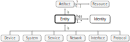
\includegraphics[scale=0.9]{figures/entity}
  \caption{
    The entity as an artifact with an identity.
    An entity or artifact may or may not be considered to be a \GlossaryHyperRef{resource}{resource}, in which case it is deemed to be valuable or useful from the perspective of a \GlossaryHyperRef{stakeholder}{stakeholder}.
    The array of artifacts with an \textit{is}-relation to \textit{Entity} is not complete.
    Other examples include \GlossaryHyperRef{cloud-local}{local clouds}, \GlossaryHyperRef{profile}{profiles} and \GlossaryHyperRef{encoding}{encodings}.
  }
  \label{fig:entity}
\end{figure}

Note that having an identity is not the same as being associated with an \GlossaryHyperRef{identifier}{identifier}, which is a name, number or other value referring to an entity.
It is enough that any such identifier is possible to produce for an artifact to count as an entity.
That being said, certain \GlossaryHyperRef{identification}{identification} requirements, perhaps related to security, performance or discoverability, may make it impractical to treat any other artifacts as entities than those with identifiers.

\subsection{Device}
\label{sec:concepts:device}

A \GlossaryHyperRef{device}{device} is a physical or \GlossaryHyperRef{virtual}{virtual} \GlossaryHyperRef{entity}{entity} with certain automation and compute \GlossaryHyperRef{capability-device}{capabilities}.
Examples of capabilities include moving robotic arms, reading from sensors, running \GlossaryHyperRef{software}{software} and sending \GlossaryHyperRef{message}{messages}.
Every device must be capable of \GlossaryHyperRef{hosting-system}{\textit{hosting}} at least one \GlossaryHyperRef{instance-software}{software} \GlossaryHyperRef{system}{system}.
Devices consist of \GlossaryHyperRef{component-hardware}{hardware components}.
When a device is \GlossaryHyperRef{device-virtual}{virtual}, its \GlossaryHyperRef{component-virtual-hardware}{hardware components} are also \GlossaryHyperRef{component-software}{software components}.
Each device must always have (1) \GlossaryHyperRef{unit-memory}{memory}, (2) \GlossaryHyperRef{unit-compute}{compute} and (3) \GlossaryHyperRef{interface-network}{network interfacing} components, as shown in Figure \ref{fig:device}.

\begin{figure}[ht!]
  \centering
  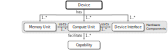
\includegraphics[scale=0.9]{figures/device}
  \caption{
    The device as a set of hardware components, each with automation or compute capabilities.
    Every device must be able to host software components using its compute and memory units, as well as communicate with other devices via its network interfaces.
    Devices with \GlossaryHyperRef{interface-human}{human interfaces} are able to communicate directly with \GlossaryHyperRef{person}{persons}.
    Other examples of hardware components could be sensors, actuators, compute accelerators and batteries.
  }
  \label{fig:device}
\end{figure}

Every device must be able to host at least one system, or it must be considered as a hardware component.
While it may seem unintuitive to consider certain machines as components, such as pumping complexes or vehicles with only manual controls, the \GlossaryHyperRef{framework-arrowhead}{Arrowhead framework} is meant to facilitate automation through the use of interconnected devices with compute capabilities.
If a machine cannot run software, making it able to host systems, that capability must be added before it can play a meaningful role in an \GlossaryHyperRef{arrowhead}{Arrowhead} context.
Consequently, machines without system hosting capabilities must be considered as components or not at all.

\subsection{System}
\label{sec:concepts:system}

A \GlossaryHyperRef{system}{system} is an \GlossaryHyperRef{identifiable}{identifiable} \GlossaryHyperRef{instance-software}{software instance} that is \GlossaryHyperRef{hosting-system}{hosted} by a \GlossaryHyperRef{device}{device}.
As shown in Figure \ref{fig:system}, a system consists of \GlossaryHyperRef{component-software}{software components}.
Just as \GlossaryHyperRef{component-hardware}{hardware components}, software components can have various types of automation or compute \GlossaryHyperRef{capability-system}{capabilities}.
Every system should have and provide at least one \GlossaryHyperRef{service}{service}, as well as have at least one \GlossaryHyperRef{interface-system}{\textit{system interface}} through which it can send and/or receive \GlossaryHyperRef{message}{messages} for its services.
If not, it must be referred to as an \GlossaryHyperRef{system-opaque}{\textit{opaque system}}.

\vspace*{-1mm}

\begin{figure}[ht!]
  \centering
  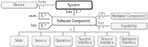
\includegraphics[scale=0.9]{figures/system}
  \caption{
    The system as a set of related software components, endowing a hosting device with new automation or compute capabilities.
    Other examples of software components could be operating systems, files, file systems, software libraries, programming language runtimes, databases and virtual machines.
  }
  \label{fig:system}
\end{figure}

Note that systems are not required to have any particular relationships to operating system processes, binary formats, virtual machines, and so on.
They may be \GlossaryHyperRef{implementation-software}{implemented} in any way deemed suitable.

\subsection{Service}
\label{sec:concepts:service}

A \GlossaryHyperRef{service}{service} is an \GlossaryHyperRef{identifiable}{identifiable} set of \GlossaryHyperRef{operation}{operations}, where each operation represents one set of activities the \GlossaryHyperRef{system}{system} \GlossaryHyperRef{provider-service}{providing} the service can perform in response to a \GlossaryHyperRef{message}{message}.
A \GlossaryHyperRef{provision-service}{provided} service always \GlossaryHyperRef{operation-exposed}{exposes} all of its operations.
Examples of activities an operation could perform include sending messages, moving robotic arms, reading value from sensors and generating a statistical reports.
For it to be possible for the service to receive messages, it must have at least one \GlossaryHyperRef{interface-service}{\textit{service interface}}, as depicted in Figure \ref{fig:service}.
When a message is received by a particular service interface, it must determine what operation to \GlossaryHyperRef{routing}{route} the message to.
This is made possible by every message being required to stating what exact operation it targets.

\begin{figure}[ht!]
  \centering
  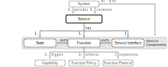
\includegraphics[scale=0.9]{figures/service}
  \caption{
    The service as a set of operations, making it possible for a providing system to offer the use of its capabilities to consuming systems via its service interfaces.
  }
  \label{fig:service}
\end{figure}

The primary reason why the service exists as a concept at all is to allow for related operations to be grouped together.
Most significantly, such groups enables the designer of an operation to require that other, complementary, operations are also made available at the same time.

\subsection{Operation}
\label{sec:concepts:operation}

An \GlossaryHyperRef{operation}{operation} is an individually \GlossaryHyperRef{identifiable}{identifiable} \GlossaryHyperRef{component-software}{component} of a \GlossaryHyperRef{service}{service} that can handle given \GlossaryHyperRef{message}{messages}.
Every operation is \GlossaryHyperRef{operation-exposed}{\textit{exposed}} via a service and may use any \GlossaryHyperRef{capability-system}{capabilities} of the \GlossaryHyperRef{system}{system} \GlossaryHyperRef{provision-service}{providing} it, as depicted in Figure \ref{fig:operation}.
Operations receive messages via \GlossaryHyperRef{interface-operation}{\textit{operation interfaces}}, which, in turn, receive them via \GlossaryHyperRef{interface-service}{service interfaces}.
If an operation needs to send messages, it may do so via the operation interfaces of \GlossaryHyperRef{stub-service}{service stubs} representing the services it targets.
How \GlossaryHyperRef{interface}{interfaces} send and receive messages is described in detail in Section \ref{sec:concepts:interface}.

\begin{figure}[ht!]
  \centering
  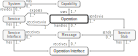
\includegraphics[scale=0.9]{figures/operation}
  \caption{
    The operation as an entity exercising the capabilities of its system in response to messages it receives via its operation interfaces, which, in turn, receives messages via service interfaces.
    Operations send messages via the operation interfaces of service stubs.
  }
  \label{fig:operation}
\end{figure}

While the operation is conceptually similar to a regular \GlossaryHyperRef{function-computer}{function} in a programming language, there are important differences.
Firstly, an operation accepts only one argument, which is a message of a well-defined \GlossaryHyperRef{type-data}{data type}.
Secondly, an operation may choose to respond the messages it receives any number of times, including not at all, at any points in time.

\newpage

\subsection{System-of-Systems}
\label{sec:concepts:sos}

A \GlossaryHyperRef{system-of-systems}{system-of-systems} is a set of at least two \GlossaryHyperRef{system}{systems} that collaborate by at least one system \GlossaryHyperRef{consumer-service}{consuming} at least one \GlossaryHyperRef{service}{service} \GlossaryHyperRef{provider-service}{provided} by another system in the same set.
The definition is depicted in Figure \ref{fig:system-of-systems}.

\begin{figure}[ht!]
  \centering
  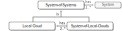
\includegraphics[scale=0.9]{figures/system-of-systems}
  \caption{
    A system-of-systems, in which at least one system consumes the service of another.
  }
  \label{fig:system-of-systems}
\end{figure}

As exemplified in Section \ref{sec:overview:system-composition}, when a system-of-systems form, its constituent systems may become able do things collectively that none of them could do on its own.
Systems-of-systems are often designed to take advantage of such \GlossaryHyperRef{capability-emergent}{emergent capabilities}.

\subsection{Cloud}
\label{sec:concepts:cloud}

A \GlossaryHyperRef{cloud}{cloud} is an \GlossaryHyperRef{identifiable}{identifiable} \GlossaryHyperRef{system-of-systems}{system-of-systems} with at least one \GlossaryHyperRef{boundary}{boundary}.
Examples of boundaries include access control policies, firewalls and gateway or border systems.
I must be possible for every system within the boundary to send messages to any other system also inside the boundary, even if the sender in question does not support any services of the receiver.
This means that for a system to be considered to be added to a cloud, it must be within its boundary and be able to communicate with all other systems inside it.
Clouds can be either \GlossaryHyperRef{cloud-local}{\textit{local}} or \GlossaryHyperRef{cloud-virtual}{\textit{virtual}}, depending on if the value they produce are bound to specific physical locations or not.
Refer to Section \ref{sec:overview:system-composition} for an overview of the differences between local and virtual clouds.

\begin{figure}[ht!]
  \centering
  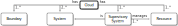
\includegraphics[scale=0.9]{figures/cloud}
  \caption{
    The cloud defined as a system-of-systems with at least one boundary.
  }
  \label{fig:cloud}
\end{figure}

A cloud could be engaged in manufacturing, repairs, heating, electricity distribution, workspace monitoring, drone fleet control, among many other possible kinds of physical activities.
A cloud may be stationary or mobile.

\subsection{System-of-Clouds}
\label{sec:concepts:soc}

A \GlossaryHyperRef{system-of-clouds}{system-of-clouds} is a set of at least two \GlossaryHyperRef{system}{clouds} that collaborate by at least one cloud \GlossaryHyperRef{consumer-service}{consuming} at least one \GlossaryHyperRef{service}{service} \GlossaryHyperRef{provider-service}{provided} by another cloud in the same set.
The definition is depicted in Figure \ref{fig:system-of-clouds}.
It is similar to the system-of-systems, with the exception of its \GlossaryHyperRef{subsystem}{subsystems} are \GlossaryHyperRef{cloud}{clouds} instead of plain \GlossaryHyperRef{system}{systems}.

\begin{figure}[ht!]
  \centering
  
\includegraphics[scale=0.9]{figures/system-of-clouds}
  \caption{
    A system-of-clouds, in which at least one cloud consumes the service of another.
  }
  \label{fig:system-of-clouds}
\end{figure}

A system-of-clouds may have its own \GlossaryHyperRef{boundary-cloud}{boundaries} in addition to those of its constituent clouds.
Those boundaries are formed by attributes shared by all the constituent local clouds, such as certificates issued by the same organization, or physical attachment to the same network bus.
A system-of-clouds cannot have resources beyond those of its constituent clouds, however.

\subsection{Network}
\label{sec:concepts:network}

A \GlossaryHyperRef{network}{network} is a set of two or more \GlossaryHyperRef{device}{devices}, \GlossaryHyperRef{connection}{connected} via \GlossaryHyperRef{interface-network}{network interfaces} such that \GlossaryHyperRef{message}{messages} can pass between them.
As shown in Figure \ref{fig:network}, devices may be \GlossaryHyperRef{interconnection}{interconnected} via \GlossaryHyperRef{device-intermediary}{intermediary devices}, examples of which could be routers, switches, hubs, busses and firewalls.
The term \GlossaryHyperRef{device-end}{\textit{end device}} may be used to represent any device not being an intermediary device.
Any technology able to connect devices is treated as facilitating networks, even if not typically associated with conventional networking methods.

\begin{figure}[ht!]
  \centering
  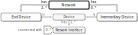
\includegraphics[scale=0.9]{figures/network}
  \caption{
    The network as a set of connected end devices, potentially interconnected via intermediary devices.
  }
  \label{fig:network}
\end{figure}

\vspace*{-4mm}

\subsection{Interface}
\label{sec:concepts:interface}

An \GlossaryHyperRef{interface}{interface} is an \GlossaryHyperRef{identifiable}{identifiable} \GlossaryHyperRef{boundary}{boundary} over which \GlossaryHyperRef{message}{messages} adhering to a supported \GlossaryHyperRef{protocol}{protocol} can cross, if those messages also satisfy all \GlossaryHyperRef{policy}{policies} associated with that interface.
From the perspective of \GlossaryHyperRef{service}{service} \GlossaryHyperRef{provision-service}{provision} and \GlossaryHyperRef{consumption-service}{consumption}, four types of interfaces are particularly relevant.
These are (1) \GlossaryHyperRef{interface-network}{network interfaces}, (2) \GlossaryHyperRef{interface-system}{system interfaces}, (3) \GlossaryHyperRef{interface-service}{service interfaces} and (4) \GlossaryHyperRef{interface-operation}{operation interfaces}, which relate as outlined in Figure \ref{fig:interface}.

\begin{figure}[ht!]
  \centering
  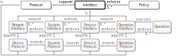
\includegraphics[scale=0.9]{figures/interface}
  \caption{
    The interface as an implemented protocols and a set of enforced policies.
    Devices, systems, services and operations have their own interface types, forming four stages through which \GlossaryHyperRef{message-inbound}{inbound messages} can be routed and \GlossaryHyperRef{message-outbound}{outbound messages} sent toward the operations they target.
  }
  \label{fig:interface}
\end{figure}

These four interface types form four conceptual stages, beginning with the network interface to the left and ending with the operation interface to the right.\footnote{
  For those familiar with the Internet \cite{rfc1122} and OSI \cite{iso7498_1} network models, the \textit{network interface} represents their \textit{transport layers}, while the \textit{system, service and operation} interfaces represent the \textit{application layer} of the Internet model and the \textit{session, presentation and application layers} of the OSI model.
  The system and service interfaces do not correspond directly to the OSI session and presentation layers.
}
When a network interface receives a message, it is \GlossaryHyperRef{routing-message}{\textit{routed}} rightwards through each stage until it reaches an \GlossaryHyperRef{operation}{operation}.
If the message is found to be \GlossaryHyperRef{message-invalid}{invalid}, \GlossaryHyperRef{message-forbidden}{forbidden} at any stage, an \GlossaryHyperRef{message-error}{error message} may be sent back to its sender by the stage in question.
The stages are conceptual in the sense that they are understood to exist even if they are not explicitly implemented.
An operation receiving a message may send its own messages via the operation interfaces of \GlossaryHyperRef{stub-service}{service stubs}, which represent other services.
Those operation interfaces pass on received messages primarily to network interfaces, but may pass them on directly to system or service interfaces when the targeted operation resides on the same device or system, respectively.

As each interface only supports a single protocol, it can only pass on messages of that protocol.
To make it possible for messages to pass between the four interface stages, each of the system, service and operation interfaces extends the protocols of the stage to its left.
This can be thought of as each stage requiring additional details to know where to route the messages they receive.
For a message to arrive at a network interface, for example, only network details are required.
To route that message to a system, the device owning the network interface must know what system the message targets, and so on.

\subsection{Protocol}
\label{sec:concepts:protocol}

A \GlossaryHyperRef{protocol}{protocol} is an \GlossaryHyperRef{identifiable}{identifiable} set of \GlossaryHyperRef{type-message}{message} and \GlossaryHyperRef{type-state}{state} types, used when formulating and interpreting \GlossaryHyperRef{message}{messages}.
The \textit{message types} describe what \GlossaryHyperRef{data}{data} messages must contain, while the \textit{state types} describe when received message are acceptable in relation to \GlossaryHyperRef{state-protocol}{states} protocol \GlossaryHyperRef{implementation}{implementations} are expected to maintain.
As shown in Figure \ref{fig:protocol}, a protocol may be defined as an \GlossaryHyperRef{protocol-extensible}{extension} of another protocol, conform to certain \GlossaryHyperRef{profile-protocol}{profiles} and use certain \GlossaryHyperRef{encoding}{encodings}.
Profiles add \GlossaryHyperRef{constraint}{constraints} to protocols, such as requiring that certain \GlossaryHyperRef{metadata}{metadata} by added to messages, while encodings are used to \GlossaryHyperRef{encode}{encode} and \GlossaryHyperRef{decode}{decode} messages.

\vfill

\begin{figure}[ht!]
  \centering
  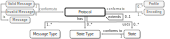
\includegraphics[scale=0.9]{figures/protocol}
  \caption{
    The protocol as set of message and state types, conforming to certain profiles and using certain encodings.
  }
  \label{fig:protocol}
\end{figure}

\vfill

Protocols are exclusively concerned with if given messages are \GlossaryHyperRef{message-valid}{valid} or \GlossaryHyperRef{message-invalid}{invalid}.
A valid message can be correctly interpreted and acted upon by the implementation of the protocol, while an invalid message cannot.
Invalid messages do not conform to all of the encodings, profiles and state types of the protocol.
Protocols are \textit{never} concerned with what messages are \GlossaryHyperRef{message-permitted}{\textit{permitted}}, which rather is the concern of the \GlossaryHyperRef{policy}{policy}.

States can be used to account for scenarios where the context in which a message is received impacts how it must be interpreted.
Consider, for example, a scenario where a \GlossaryHyperRef{service}{service} is provided for opening and closing a door.
Let us assume that the door is currently open, and a message is received by the service that instructs it to open it.
As the door is already open, it cannot be opened any more than it already is.
The message could, therefore, either be interpreted as being already handled or be rejected, depending on what the use case makes most relevant.
If the protocol of the message would not have accounted for the state of the door, open and close messages would have to always be accepted.

\subsection{Message}
\label{sec:concepts:message}

A \GlossaryHyperRef{message}{message} is \GlossaryHyperRef{data}{data} that \GlossaryHyperRef{identification}{identifies} an \GlossaryHyperRef{operation}{operation}, among any other \GlossaryHyperRef{metadata}{metadata}, any may include a payload, as depicted in Figure \ref{fig:message}.
In other words, a message describes how it is to be sent to a particular operation, made available by a particular \GlossaryHyperRef{service}{service}, \GlossaryHyperRef{system}{system} and \GlossaryHyperRef{device}{device}, as well as including any payload necessary for that operation to be able to execute as intended.

\vfill

\begin{figure}[ht!]
  \centering
  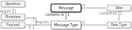
\includegraphics[scale=0.9]{figures/message}
  \caption{
    The message as data that must include metadata targeting an operation, as well as a payload.
  }
  \label{fig:message}
\end{figure}

\vfill

The metadata of a message specify the details required for it to arrive at the operation it targets, as well as additional details required to interpret the message and its payload correctly, such as by stating what \GlossaryHyperRef{encoding}{encodings} are used.
The metadata may also include details required to satisfy the \GlossaryHyperRef{policy}{policies} of the interfaces that must be passed on its journey to its target operation.
Metadata may be added, modified and/or used by \GlossaryHyperRef{interface}{interfaces} when messages pass through them.

\newpage

\subsection{Policy}
\label{sec:concepts:policy}

A \GlossaryHyperRef{policy}{policy} is an \GlossaryHyperRef{identifiable}{identifiable} set of \GlossaryHyperRef{constraint-policy}{constraints}, useful for determining if given \GlossaryHyperRef{message}{messages} are \GlossaryHyperRef{message-permitted}{permitted} or \GlossaryHyperRef{message-forbidden}{forbidden}, as depicted in Figure \ref{fig:policy}.
Policies may be concerned with authorization, contracts, economic goals, and so on.

\begin{figure}[ht!]
  \centering
  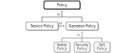
\includegraphics[scale=0.9]{figures/policy}
  \caption{
    The policy as a set of constraints, useful for determining if messages are permitted or not.
  }
  \label{fig:policy}
\end{figure}

Every policy may, when relevant, be regarded as a \GlossaryHyperRef{function-predicate}{predicate function} useful for testing if given message is permitted with respect to any kind of information.
Policies are typically enforced by \GlossaryHyperRef{interface}{interfaces}, as described in Section \ref{sec:concepts:interface}.
If a \GlossaryHyperRef{message}{message} is forbidden with respect to one or more of the policies of an interface, those policies should be listed in any error message returned to the sender of that message.

While \GlossaryHyperRef{protocol}{protocols} help determine if a given message can be passed on or interpreted correctly, \textit{policies} are meant to determine if the activity described by that message would occur under desirable conditions.
For example, an interface may receive a message requesting that a certain pump be started.
While the interpretation of the message may be clear, there may still be other conditions that make it undesirable for the pump to activate.
If the pump is on fire, turning it on may present a safety hazard; if the system attempting to start the pump is unauthorized, the risk is higher for sabotage and other wasteful behaviors; and so on.

\subsection{Profile}
\label{sec:concepts:profile}

A \GlossaryHyperRef{profile}{profile} is a set of \GlossaryHyperRef{constraint}{constraints} that can be added to a \GlossaryHyperRef{protocol}{protocol}.
A profile may require that certain flags, headers, or other \GlossaryHyperRef{metadata}{metadata}, are included in the messages of the protocols that conform to it, among other possible examples.
While a protocol may only extend up to one other protocol, it may conform to any number of profiles.
The \GlossaryHyperRef{constraint-profile}{constraints} of a profile must be based on a protocol extended by every protocol conforming to that profile, as we show in Figure \ref{fig:profile}.

\begin{figure}[ht!]
  \centering
  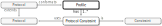
\includegraphics[scale=0.9]{figures/profile}
  \caption{
    The profile as a set of protocol constraints, which may, for example, be concerned with protocols or encodings.
    \textit{Protocol'} represents any protocol that \textit{Protocol} could extend, directly or by any extended protocol.
  }
  \label{fig:profile}
\end{figure}

While perhaps a bit difficult to grasp initially, unless this was the case there would not be anything to base the constraints on.
Consider, for example, a \GlossaryHyperRef{service}{service} with an \GlossaryHyperRef{interface-service}{interface} that supports a custom extension of the HTTP protocol \cite{fielding2014hypertext}.
Such an extended HTTP protocol could, among other things, specify how one would formulate request lines to target the \GlossaryHyperRef{operation}{operations} of the service.
An example of such a request line could be \texttt{GET /pump-7b/pressures/a14 HTTP/1.1}, which we can imagine targets an operation that fetches a pressure value from a pump.
If our custom protocol is meant to be conformant to a certain profile, the constraints of that profile must be formulated in terms of HTTP without the extension of the service interface.
As HTTP extends TCP \cite{postel1981transmission} and IP \cite{deering2017internet}, our constraints may also target details of those protocols.
An example profile could require that certain HTTP headers be included in every message, or that certain TCP flags not be used, among many other possible examples.

\subsection{Encoding}
\label{sec:concepts:encoding}

An \textit{encoding} is a \GlossaryHyperRef{type-data}{data type} that makes up a language or structure in which \GlossaryHyperRef{data}{data} can be formulated and interpreted.
The term is typically only used when considering \GlossaryHyperRef{encoder}{encoders} and \GlossaryHyperRef{decoder}{decoders}, which transform data from being expressed in one encoding into another.
More specifically, an \textit{encoder} turns data from an encoding suitable for processing into another suitable for transmission and/or storage, while a \textit{decoder} performs the reverse operation.
How encodings, encoders and decoders relate is depicted in Figure \ref{fig:encoding}.

\vfill

\begin{figure}[ht!]
  \centering
  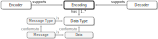
\includegraphics[scale=0.9]{figures/encoding}
  \caption{
    The encoding as a data type, supported by certain encoders and decoders.
    The \GlossaryHyperRef{compression}{compression} and the \GlossaryHyperRef{encryption}{encryption} are treated as special kinds of encodings.
  }
  \label{fig:encoding}
\end{figure}

\vfill

An encoding useful for \textit{transmission} could, for example, be JSON \cite{rfc7159},\footnote{
  The data type of the JSON encoding is a union type of seven variants: \textit{object}, \textit{array}, \textit{string}, \textit{number}, \textit{true}, \textit{false} and \textit{null}.
  Other encodings provide other data types.
  The data type of XML \cite{w3c2008xml} is, for example, its \textit{document} type, which in turn uses \textit{elements}, \textit{texts} and other types.
} while an encoding useful for \textit{storage} could be some kind of file or database format.
An encoding useful for \textit{processing} could be the binary format employed by a \GlossaryHyperRef{unit-compute}{compute unit}, virtual machine or computer language runtime, among other possible examples.

There are two kinds of encodings that deserve special attention.
These are \textit{compressions} and \textit{encryptions}.
While perhaps not often treated as if being encodings, they do fit the description of encoding we have just presented.
They transform data, often treated as plain byte arrays irrespective of their original structures, from a form suitable for processing into another form suitable for transmission and/or storage, and vice versa.
However, they differ from other encodings in that the transmission and storage form of the data is expected to gain special properties, namely to require less space or become undecipherable without knowledge of specific secrets.

\subsubsection{Compression}
\label{sec:concepts:encoding:compression}

A \GlossaryHyperRef{compression}{compression} is an \GlossaryHyperRef{encoding}{encoding} used to make \GlossaryHyperRef{data}{data} representable using less \GlossaryHyperRef{datum}{datums} during transmission or storage, which can improve performance by requiring less transmission time or storage space.
Once \GlossaryHyperRef{compress}{compressed}, the data typically cannot be interpreted in any meaningful way.
To use the data again, it must first be \GlossaryHyperRef{decompress}{decompressed}, which restores it to its original form, or some approximation of its original form.
Compressions that can restore data to their original forms are often referred to as being \textit{lossless}, while those that deal with approximations are referred to as being \textit{lossy}.
Lossy compressions are typically used for images, audio, video and other media, while lossless compression is typically used for \GlossaryHyperRef{message}{messages}.

\subsubsection{Encryption}
\label{sec:concepts:encoding:encryption}

An \GlossaryHyperRef{encryption}{encryption} is an \GlossaryHyperRef{encoding}{encoding} used to turn \GlossaryHyperRef{data}{data} into a form that cannot be interpreted by a third party during its transmission or storage.
Once \GlossaryHyperRef{encrypt}{encrypted}, there should be no practically computable means of reverting, or \GlossaryHyperRef{decrypt}{decrypting}, the data to its original form.
To make it possible for the owner of the data, or its intended receiver, to revert it back to its original form, some form of secret numbers, passwords or other keys are typically used.

Encryption is the means through which \GlossaryHyperRef{system-of-systems}{systems-of-systems} can be made secure.
It facilitates security in the sense that it makes it practically possible to guarantee the privacy, integrity and authenticity of transmitted \GlossaryHyperRef{message}{messages} and other stored data.

\newpage

\subsection{Semantics}
\label{sec:concepts:semantics}

A \GlossaryHyperRef{semantics}{semantics} is a \GlossaryHyperRef{model}{model} used to derive meaning from \GlossaryHyperRef{data}{data}.
More specifically, it \textit{disambiguates}, or makes the interpretation clear, of data conforming to any out of one or more \GlossaryHyperRef{type-data}{data types}, as illustrated in Figure \ref{fig:semantics}.
All data that are known to conform to any of these data types then become possible to interpret.
In other words, unless you are able to associate a given data type with a semantics, you cannot understand or act on any data conforming to the type.

\begin{figure}[ht!]
  \centering
  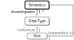
\includegraphics[scale=0.9]{figures/semantics}
  \caption{
    The semantics as a model used to disambiguate data types, making it possible to interpret data conforming to those types.
  }
  \label{fig:semantics}
\end{figure}

All data types disambiguated by the same semantics must express the same intrinsic meaning.
Consider, for example, the JSON \cite{rfc7159} object \texttt{\{"v":21.30\}} and the XML \cite{w3c2008xml} element \texttt{<rd temp=70.34/>}.
Both of these are data, both of them conform to a data type, and both of those data types conform to the same semantics.
The JSON object represents a temperature value in celsius and the XML element represents the same temperature expressed in fahrenheit.
Despite having the same semantics, however, their structures are quite different.

\subsubsection{Semantics Profile}
\label{sec:concepts:semantics:profile}

When a semantics disambiguates two or more data types, it can be used to construct a \GlossaryHyperRef{profile-semantic}{semantic profile}.
Such a \GlossaryHyperRef{profile}{profile} requires that the every conformant \GlossaryHyperRef{protocol}{protocol} has a relevant \GlossaryHyperRef{encoding}{encoding} whose data type is disambiguated by a certain semantics.

A common application of semantic profiles is to make different protocols express the same meanings, even though they use different encodings.
For example, a certain protocol may be based on HTTP \cite{fielding2014hypertext} and JSON \cite{rfc7159}, while another is based on CoAP \cite{rfc7252} and CBOR \cite{rfc8949}.
If the payloads of both protocols would conform to the same semantic profile, the messages of both protocols would express the same intents and meanings despite being structured differently.
